\documentclass[unknownkeysallowed]{beamer}

\usepackage[utf8]{inputenc}
\usepackage{lmodern}

\setcounter{tocdepth}{2}

\usepackage{listings}

% For For-Loops
\usepackage{forloop}
\newcounter{ct}

\usepackage{graphicx}
\usepackage{xcolor}
\usepackage{tikz}
\usetikzlibrary{arrows, snakes, backgrounds}
\usepackage{wrapfig}

\setbeamercovered{transparent}
% for \uptau
\usepackage{upgreek}

\title{Rate Monotonic vs. EDF: Judgment Day}
\subtitle{von Buttazzo, G. C.}
\date{\today}
\author{Dominik Schlecht}
\institute[THI]{Technische Hochschule Ingolstadt}

\usetheme{Copenhagen}

% Fix ToC-Spacing
\usepackage{etoolbox}

\makeatletter
\patchcmd{\beamer@sectionintoc}{\vskip1.5em}{\vskip0.5em}{}{}
\makeatother

\AtBeginSubsection[]
%\AtBeginSection[]
{
	\begin{frame}<beamer>
		\frametitle{Gliederung}
		\tableofcontents[
  			currentsection,
  			sectionstyle=show/show,
  			subsectionstyle=show/shaded/hide,
  			squeeze
		]
	\end{frame}
}

% Document..
\begin{document}
	\frame{\maketitle}
	\frame{\tableofcontents[hideallsubsections]}
	
	
	\section{Einleitung}
	\subsection{Meta-Informationen}
\begin{frame}{\subsecname}
	\begin{itemize}
		\item Author:
		\begin{itemize}
			\item Giorgio C. Buttazzo
			\item University of Pavia, Italien
			\item buttazzo@unipv.it
		\end{itemize}\pause
		\item Whitepaper
		\begin{itemize}
			\item Rate Monotonic vs. EDF: Judgment Day
			\item Real-Time Systems, 29, 5–26, 2005
		\end{itemize}						
		
	\end{itemize}
\end{frame} 

\subsection{Abstract}
\begin{frame}{\subsecname}
\tiny Since the first results published in 1973 by Liu and Layland on the Rate Monotonic (RM) and Earliest Deadline First (EDF) algorithms, a lot of progress has been made in the schedulability analysis of periodic task sets. Unfortunately, many misconceptions still exist about the properties of these two scheduling methods, which usually tend to favor RM more than EDF. Typical wrong statements often heard in technical conferences and even in research papers claim that RM is easier to analyze than EDF, it introduces less runtime overhead, it is more predictable in overload conditions, and causes less jitter in task execution.Since the above statements are either wrong, or not precise \tiny, it is time to clarify these issues in a systematic fashion, because the use of EDF allows a better exploitation of the available resources and significantly improves system’s performance. This paper compares RM against EDF under several aspects, using existing theoretical results, specific simulation experiments, or simple counterexamples to show that many common beliefs are either false or only restricted to specific situations.\footnote{Rate Monotonics vs. EDF: Judgment Day, Girorgio C. Buttazzo, 2005}
\end{frame}

\begin{frame}{\subsecname}
	\begin{center}
		
\includegraphics[scale=0.25]{graphics/memes/aintnobody.jpg}
	\end{center}
\end{frame}

\begin{frame}{\subsecname}
\tiny Since the first results published in 1973 by Liu and Layland on the Rate Monotonic (RM) and Earliest Deadline First (EDF) algorithms, a lot of progress has been made in the schedulability analysis of periodic task sets. Unfortunately, many misconceptions still exist about the properties of these two scheduling methods, which usually tend to favor RM more than EDF. Typical wrong statements often heard in technical conferences and even in research papers claim that RM is easier to analyze than EDF, it introduces less runtime overhead, it is more predictable in overload conditions, and causes less jitter in task execution.Since the above statements are either wrong, or not precise \tiny, it is time to clarify these issues in a systematic fashion, because the use of EDF allows a better exploitation of the available resources and significantly improves system’s performance. This paper compares RM against EDF under several aspects, using existing theoretical results, specific simulation experiments, or simple counterexamples to show that many common beliefs are either false or only restricted to specific situations.\footnote{Rate Monotonics vs. EDF: Judgment Day, Girorgio C. Buttazzo, 2005}
\end{frame}

\begin{frame}{\subsecname}
\tiny Since the first results published in 1973 by Liu and Layland on the Rate Monotonic (RM) and Earliest Deadline First (EDF) algorithms, a lot of progress has been made in the schedulability analysis of periodic task sets. Unfortunately, many \Large misconceptions \tiny still exist about the properties of these two scheduling methods, which usually tend to favor RM more than EDF. Typical wrong statements often heard in technical conferences and even in research papers claim that RM is easier to analyze than EDF, it introduces less runtime overhead, it is more predictable in overload conditions, and causes less jitter in task execution.Since the above statements are either wrong, or not precise, it is time to clarify these issues in a systematic fashion, because the use of EDF allows a better exploitation of the available resources and significantly improves system’s performance. This paper compares RM against EDF under several aspects, using existing theoretical results, specific simulation experiments, or simple counterexamples to show that many common beliefs are either false or only restricted to specific situations.\footnote{Rate Monotonics vs. EDF: Judgment Day, Girorgio C. Buttazzo, 2005}
\end{frame}
	
\begin{frame}{\subsecname}
\tiny Since the first results published in 1973 by Liu and Layland on the Rate Monotonic (RM) and Earliest Deadline First (EDF) algorithms, a lot of progress has been made in the schedulability analysis of periodic task sets. Unfortunately, many \Large misconceptions \tiny still exist about the properties of these two scheduling methods, which usually tend to \Large favor RM more than EDF \tiny. Typical wrong statements often heard in technical conferences and even in research papers claim that RM is easier to analyze than EDF, it introduces less runtime overhead, it is more predictable in overload conditions, and causes less jitter in task execution.Since the above statements are either wrong, or not precise, it is time to clarify these issues in a systematic fashion, because the use of EDF allows a better exploitation of the available resources and significantly improves system’s performance. This paper compares RM against EDF under several aspects, using existing theoretical results, specific simulation experiments, or simple counterexamples to show that many common beliefs are either false or only restricted to specific situations.\footnote{Rate Monotonics vs. EDF: Judgment Day, Girorgio C. Buttazzo, 2005}
\end{frame}

	\begin{frame}{\subsecname}
\tiny Since the first results published in 1973 by Liu and Layland on the Rate Monotonic (RM) and Earliest Deadline First (EDF) algorithms, a lot of progress has been made in the schedulability analysis of periodic task sets. Unfortunately, many \Large misconceptions \tiny still exist about the properties of these two scheduling methods, which usually tend to \Large favor RM more than EDF \tiny. Typical wrong statements often heard in technical conferences and even in research papers claim that RM is easier to analyze than EDF, it introduces less runtime overhead, it is more predictable in overload conditions, and causes less jitter in task execution.Since the above statements are \Large  either wrong, or not precise \tiny, it is time to clarify these issues in a systematic fashion, because the use of EDF allows a better exploitation of the available resources and significantly improves system’s performance. This paper compares RM against EDF under several aspects, using existing theoretical results, specific simulation experiments, or simple counterexamples to show that many common beliefs are either false or only restricted to specific situations.\footnote{Rate Monotonics vs. EDF: Judgment Day, Girorgio C. Buttazzo, 2005}
\end{frame}
	
\begin{frame}{\subsecname}
\tiny Since the first results published in 1973 by Liu and Layland on the Rate Monotonic (RM) and Earliest Deadline First (EDF) algorithms, a lot of progress has been made in the schedulability analysis of periodic task sets. Unfortunately, many \Large misconceptions \tiny still exist about the properties of these two scheduling methods, which usually tend to \Large favor RM more than EDF \tiny. Typical wrong statements often heard in technical conferences and even in research papers claim that RM is easier to analyze than EDF, it introduces less runtime overhead, it is more predictable in overload conditions, and causes less jitter in task execution.Since the above statements are \Large  either wrong, or not precise \tiny, it is time to clarify these issues in a systematic fashion, because the use of EDF allows a better exploitation of the available resources and significantly improves system’s performance. \Large This paper compares RM against EDF \tiny under several aspects, using existing theoretical results, specific simulation experiments, or simple counterexamples to show that many common beliefs are either false or only restricted to specific situations.\footnote{Rate Monotonics vs. EDF: Judgment Day, Girorgio C. Buttazzo, 2005}
\end{frame}


\begin{frame}{\subsecname}
	\begin{center}
		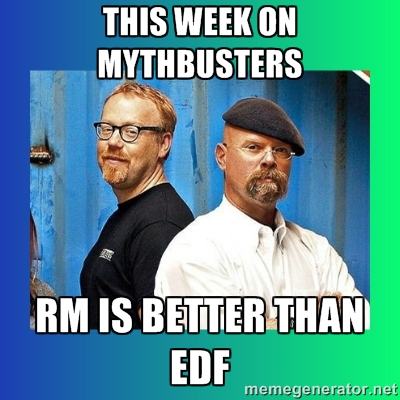
\includegraphics[scale=0.6]{graphics/memes/mythbusters_thisweek.jpg}
	\end{center}
\end{frame}

%\section{Erläuterung}
\subsection{Flashback - Scheduling}
\begin{frame}{\subsecname}
	Wir definieren:
	\begin{equation}
		\uptau_{i, k} \text{ als Job mit einer absoluten Deadline } d_{i, k}
	\end{equation}
	\pause
	\begin{equation}
		\uptau_i \text{ als infinite Folge von Jobs } \uptau_{i, k} \text{ mit }
	\end{equation}
	\pause
	\begin{equation}
		\begin{array}{l l l}
			\text{Wort-Case-Execution-Time } & C_i\\
			\text{Task-Period } & T_i
		\end{array}
	\end{equation}
\end{frame}

\begin{frame}{\subsecname}
	\begin{center}
		%\rowcolors{1}{RoyalBlue!20}{RoyalBlue!5}
		\begin{tabular}{c||c|c}
			Task ($\uptau_i$) & Dauer ($C_i$) & Task-Periode ($T_i$)\\\hline\hline
			$\uptau_1$ & 5 & 15
		\end{tabular}
	\end{center}
	\begin{figure}[htbp]
	% Partly taken from http://www.texample.net/tikz/examples/convolution-of-two-functions/
	\centering
	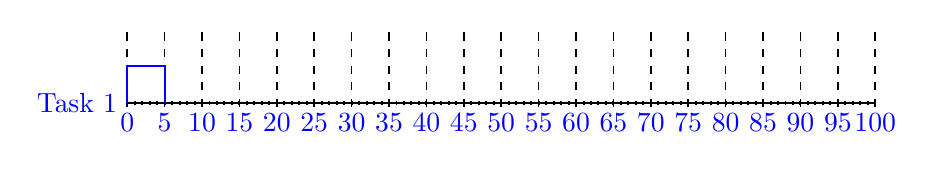
\begin{tikzpicture}[
		scale=0.095,
		line width=0.25mm,
		every node/.style={scale=1, text=blue},
		major tick/.style={semithick, dashed},
		x tick label/.style={anchor=north, minimum width=5mm},
		task1/.style={blue},
		task2/.style={red},
		task3/.style={green},
		desc/.style={anchor=east}
		]
	
	% Task 1
	\draw (0, 0) -- (100, 0);
	\node[desc] at (0, 0) {Task 1};
	
%	% Task 2
%	\draw (0, 10) -- (100, 10);
%	\node[desc] at (0, 10) {Task 2};	
%	
%	% Task 3
%	\draw (0, 20) -- (100, 20);
%	\node[desc] at (0, 20) {Task 3};	
	
	% Small ticks
	\foreach \x in {0, 1,...,100}{
		\draw (\x, -0.25) -- (\x, 0.25);
	}
	
	% Major ticks with label
	\foreach \x/\label in {0, 5,...,100}{
		\node[x tick label] at (\x, 0) {$\label$}; 		
		\draw[major tick] (\x, -0.5) -- (\x, 10);
	}
	
	% Draw all
%	\foreach \x in {0, 15,...,100}{
%		\draw[task1] (\x, 0) -- (\x, 5) -- (\x+5, 5) -- (\x+5, 0);
%	}
	
	% Single steps for the slides
	\draw[task1] (0, 0) -- (0, 5) -- (5, 5) -- (5, 0);
%	\draw[task1] (15, 0) -- (15, 5) -- (20, 5) -- (20, 0);
%	\draw[task1] (30, 0) -- (30, 5) -- (35, 5) -- (35, 0);
%	\draw[task1] (45, 0) -- (45, 5) -- (50, 5) -- (50, 0);
%	\draw[task1] (60, 0) -- (60, 5) -- (65, 5) -- (65, 0);
%	\draw[task1] (75, 0) -- (75, 5) -- (80, 5) -- (80, 0);
%	\draw[task1] (90, 0) -- (90, 5) -- (95, 5) -- (95, 0);

	\end{tikzpicture}
\end{figure}
\end{frame}

\begin{frame}{\subsecname}
	\begin{center}
		%\rowcolors{1}{RoyalBlue!20}{RoyalBlue!5}
		\begin{tabular}{c||c|c}
			Task ($\uptau_i$) & Dauer ($C_i$) & Task-Periode ($T_i$)\\\hline\hline
			$\uptau_1$ & 5 & 15
		\end{tabular}
	\end{center}
	\begin{figure}[htbp]
	% Partly taken from http://www.texample.net/tikz/examples/convolution-of-two-functions/
	\centering
	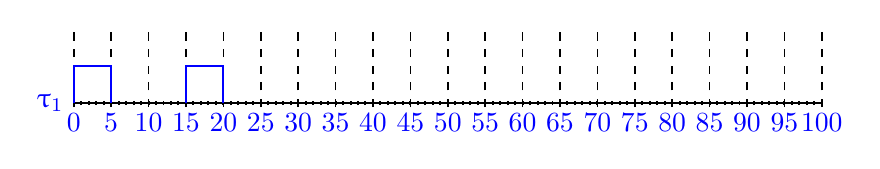
\begin{tikzpicture}[
		scale=0.095,
		line width=0.25mm,
		every node/.style={scale=1, text=blue},
		major tick/.style={semithick, dashed},
		x tick label/.style={anchor=north, minimum width=5mm},
		task1/.style={blue},
		task2/.style={red},
		task3/.style={green},
		desc/.style={anchor=east}
		]
	
	% Task 1
	\draw (0, 0) -- (100, 0);
	\node[desc] at (0, 0) {$\uptau_1$};
	
%	% Task 2
%	\draw (0, 10) -- (100, 10);
%	\node[desc] at (0, 10) {Task 2};	
%	
%	% Task 3
%	\draw (0, 20) -- (100, 20);
%	\node[desc] at (0, 20) {Task 3};	
	
	% Small ticks
	\foreach \x in {0, 1,...,100}{
		\draw (\x, -0.25) -- (\x, 0.25);
	}
	
	% Major ticks with label
	\foreach \x/\label in {0, 5,...,100}{
		\node[x tick label] at (\x, 0) {$\label$}; 		
		\draw[major tick] (\x, -0.5) -- (\x, 10);
	}
	
	% Draw all
%	\foreach \x in {0, 15,...,100}{
%		\draw[task1] (\x, 0) -- (\x, 5) -- (\x+5, 5) -- (\x+5, 0);
%	}
	
	% Single steps for the slides
	\draw[task1] (0, 0) -- (0, 5) -- (5, 5) -- (5, 0);
	\draw[task1] (15, 0) -- (15, 5) -- (20, 5) -- (20, 0);
%	\draw[task1] (30, 0) -- (30, 5) -- (35, 5) -- (35, 0);
%	\draw[task1] (45, 0) -- (45, 5) -- (50, 5) -- (50, 0);
%	\draw[task1] (60, 0) -- (60, 5) -- (65, 5) -- (65, 0);
%	\draw[task1] (75, 0) -- (75, 5) -- (80, 5) -- (80, 0);
%	\draw[task1] (90, 0) -- (90, 5) -- (95, 5) -- (95, 0);

	\end{tikzpicture}
\end{figure}
\end{frame}

\begin{frame}{\subsecname}
	\begin{center}
		%\rowcolors{1}{RoyalBlue!20}{RoyalBlue!5}
		\begin{tabular}{c||c|c}
			Task ($\uptau_i$) & Dauer ($C_i$) & Task-Periode ($T_i$)\\\hline\hline
			$\uptau_1$ & 5 & 15
		\end{tabular}
	\end{center}
	\begin{figure}[htbp]
	% Partly taken from http://www.texample.net/tikz/examples/convolution-of-two-functions/
	\centering
	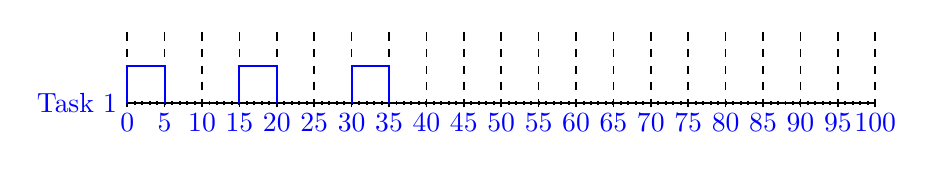
\begin{tikzpicture}[
		scale=0.095,
		line width=0.25mm,
		every node/.style={scale=1, text=blue},
		major tick/.style={semithick, dashed},
		x tick label/.style={anchor=north, minimum width=5mm},
		task1/.style={blue},
		task2/.style={red},
		task3/.style={green},
		desc/.style={anchor=east}
		]
	
	% Task 1
	\draw (0, 0) -- (100, 0);
	\node[desc] at (0, 0) {Task 1};
	
%	% Task 2
%	\draw (0, 10) -- (100, 10);
%	\node[desc] at (0, 10) {Task 2};	
%	
%	% Task 3
%	\draw (0, 20) -- (100, 20);
%	\node[desc] at (0, 20) {Task 3};	
	
	% Small ticks
	\foreach \x in {0, 1,...,100}{
		\draw (\x, -0.25) -- (\x, 0.25);
	}
	
	% Major ticks with label
	\foreach \x/\label in {0, 5,...,100}{
		\node[x tick label] at (\x, 0) {$\label$}; 		
		\draw[major tick] (\x, -0.5) -- (\x, 10);
	}
	
	% Draw all
%	\foreach \x in {0, 15,...,100}{
%		\draw[task1] (\x, 0) -- (\x, 5) -- (\x+5, 5) -- (\x+5, 0);
%	}
	
	% Single steps for the slides
	\draw[task1] (0, 0) -- (0, 5) -- (5, 5) -- (5, 0);
	\draw[task1] (15, 0) -- (15, 5) -- (20, 5) -- (20, 0);
	\draw[task1] (30, 0) -- (30, 5) -- (35, 5) -- (35, 0);
%	\draw[task1] (45, 0) -- (45, 5) -- (50, 5) -- (50, 0);
%	\draw[task1] (60, 0) -- (60, 5) -- (65, 5) -- (65, 0);
%	\draw[task1] (75, 0) -- (75, 5) -- (80, 5) -- (80, 0);
%	\draw[task1] (90, 0) -- (90, 5) -- (95, 5) -- (95, 0);

	\end{tikzpicture}
\end{figure}
\end{frame}

\begin{frame}{\subsecname}
	\begin{center}
		%\rowcolors{1}{RoyalBlue!20}{RoyalBlue!5}
		\begin{tabular}{c||c|c}
			Task ($\uptau_i$) & Dauer ($C_i$) & Task-Periode ($T_i$)\\\hline\hline
			$\uptau_1$ & 5 & 15
		\end{tabular}
	\end{center}
	\begin{figure}[htbp]
	% Partly taken from http://www.texample.net/tikz/examples/convolution-of-two-functions/
	\centering
	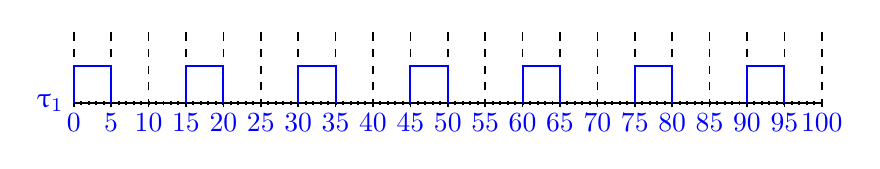
\begin{tikzpicture}[
		scale=0.095,
		line width=0.25mm,
		every node/.style={scale=1, text=blue},
		major tick/.style={semithick, dashed},
		x tick label/.style={anchor=north, minimum width=5mm},
		task1/.style={blue},
		task2/.style={red},
		task3/.style={green},
		desc/.style={anchor=east}
		]
	
	% Task 1
	\draw (0, 0) -- (100, 0);
	\node[desc] at (0, 0) {$\uptau_1$};
	
%	% Task 2
%	\draw (0, 10) -- (100, 10);
%	\node[desc] at (0, 10) {Task 2};	
%	
%	% Task 3
%	\draw (0, 20) -- (100, 20);
%	\node[desc] at (0, 20) {Task 3};	
	
	% Small ticks
	\foreach \x in {0, 1,...,100}{
		\draw (\x, -0.25) -- (\x, 0.25);
	}
	
	% Major ticks with label
	\foreach \x/\label in {0, 5,...,100}{
		\node[x tick label] at (\x, 0) {$\label$}; 		
		\draw[major tick] (\x, -0.5) -- (\x, 10);
	}
	
	% Draw all
%	\foreach \x in {0, 15,...,100}{
%		\draw[task1] (\x, 0) -- (\x, 5) -- (\x+5, 5) -- (\x+5, 0);
%	}
	
	% Single steps for the slides
	\draw[task1] (0, 0) -- (0, 5) -- (5, 5) -- (5, 0);
	\draw[task1] (15, 0) -- (15, 5) -- (20, 5) -- (20, 0);
	\draw[task1] (30, 0) -- (30, 5) -- (35, 5) -- (35, 0);
	\draw[task1] (45, 0) -- (45, 5) -- (50, 5) -- (50, 0);
	\draw[task1] (60, 0) -- (60, 5) -- (65, 5) -- (65, 0);
	\draw[task1] (75, 0) -- (75, 5) -- (80, 5) -- (80, 0);
	\draw[task1] (90, 0) -- (90, 5) -- (95, 5) -- (95, 0);

	\end{tikzpicture}
\end{figure}
\end{frame}

\begin{frame}{\subsecname}
	\begin{center}
		\begin{tabular}{c||c|c}
				Task ($\uptau_i$) & Dauer ($C_i$) & Task-Periode ($T_i$)\\\hline\hline
				$\uptau_1$ & 5 & 15\\
				$\uptau_2$ & 10 & 40\\
		\end{tabular}
	\end{center}	
	\begin{figure}[htbp]
	% Partly taken from http://www.texample.net/tikz/examples/convolution-of-two-functions/
	\centering
	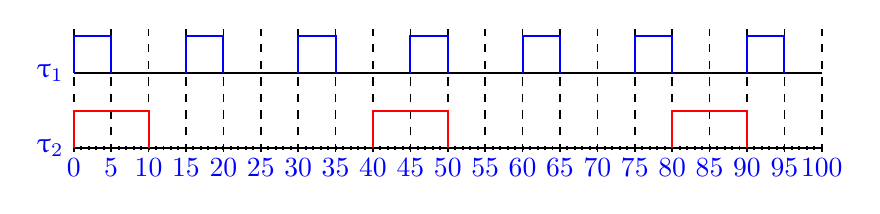
\begin{tikzpicture}[
		scale=0.095,
		line width=0.25mm,
		every node/.style={scale=1, text=blue},
		major tick/.style={semithick, dashed},
		x tick label/.style={anchor=north, minimum width=5mm},
		task1/.style={blue},
		task2/.style={red},
		task3/.style={green},
		desc/.style={anchor=east}
		]

	% Task 1
	\draw (0, 10) -- (100, 10);
	\node[desc] at (0, 10) {$\uptau_1$};
	
	% Task 2
	\draw (0, 0) -- (100, 0);
	\node[desc] at (0, 0) {$\uptau_2$};	
	
	% Small ticks
	\foreach \x in {0, 1,...,100}{
		\draw (\x, -0.25) -- (\x, 0.25);
	}
	
	% Major ticks with label
	\foreach \x/\label in {0, 5,...,100}{
		\node[x tick label] at (\x, 0) {$\label$}; 		
		\draw[major tick] (\x, -0.5) -- (\x, 16);
	}
	
	% Draw all Task 1
	\foreach \x in {0, 15,...,100}{
		\draw[task1] (\x, 10) -- (\x, 15) -- (\x+5, 15) -- (\x+5, 10);
	}
	
	% Draw all Task 2
	\foreach \x in {0, 40,...,100}{
		\draw[task2] (\x, 0) -- (\x, 5) -- (\x+10, 5) -- (\x+10, 0);
	}
	
	\end{tikzpicture}
\end{figure}
\end{frame}

\begin{frame}{\subsecname}
	\begin{center}
		\begin{tabular}{c||c|c}
				Task ($\uptau_i$) & Dauer ($C_i$) & Task-Periode ($T_i$)\\\hline\hline
				$\uptau_1$ & 5 & 15\\
				$\uptau_2$ & 10 & 40\\
		\end{tabular}
	\end{center}	
	\begin{figure}[htbp]
	% Partly taken from http://www.texample.net/tikz/examples/convolution-of-two-functions/
	\centering
	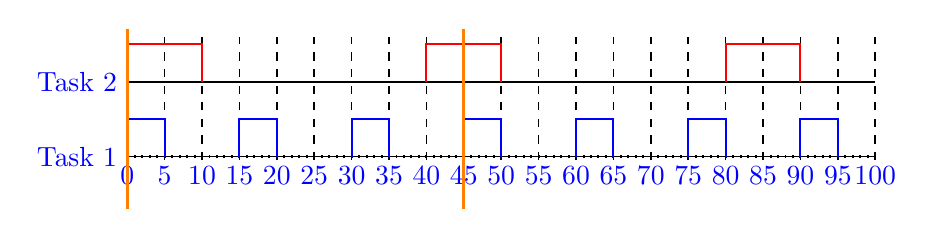
\begin{tikzpicture}[
		scale=0.095,
		line width=0.25mm,
		every node/.style={scale=1, text=blue},
		major tick/.style={semithick, dashed},
		x tick label/.style={anchor=north, minimum width=5mm},
		task1/.style={blue},
		task2/.style={red},
		task3/.style={green},
		desc/.style={anchor=east},
		konf/.style={orange, very thick}
		]
	
	% Task 1
	\draw (0, 0) -- (100, 0);
	\node[desc] at (0, 0) {Task 1};
	
	% Task 2
	\draw (0, 10) -- (100, 10);
	\node[desc] at (0, 10) {Task 2};	
%	
%	% Task 3
%	\draw (0, 20) -- (100, 20);
%	\node[desc] at (0, 20) {Task 3};	
	
	% Small ticks
	\foreach \x in {0, 1,...,100}{
		\draw (\x, -0.25) -- (\x, 0.25);
	}
	
	% Major ticks with label
	\foreach \x/\label in {0, 5,...,100}{
		\node[x tick label] at (\x, 0) {$\label$}; 		
		\draw[major tick] (\x, -0.5) -- (\x, 16);
	}
	
	% Draw all
	\foreach \x in {0, 15,...,100}{
		\draw[task1] (\x, 0) -- (\x, 5) -- (\x+5, 5) -- (\x+5, 0);
	}
	
	% Draw all
	\foreach \x in {0, 40,...,100}{
		\draw[task2] (\x, 10) -- (\x, 15) -- (\x+10, 15) -- (\x+10, 10);
	}
	
	\draw[konf] (0, 17) -- (0, -7);
	\draw[konf] (45, 17) -- (45, -7);
	
	\end{tikzpicture}
\end{figure}
\end{frame}

	
	\section{Rate Monotonic \& Erliest Deadline First}
	\subsection{Grundlagen}
\begin{frame}{\subsecname}
		\begin{columns}[]
  			\begin{column}{0.5\textwidth}
				Rate Monotonics:
				\begin{itemize}
					\item Job $T_{i, k}$ mit kürzester Periode wird bevorzugt
					\item Task $T_i$ wird anfangs eine Priorität zugewiesen
				\end{itemize}

			\end{column}
  			\begin{column}{0.5\textwidth}
  				Erliest Deadline First:
				\begin{itemize}
					\item Job $T_{i, k}$ mit der nächsten Deadline wird bevorzugt
					\item Die Priorität von Task $T_i$ entscheidet sich während der Laufzeit
				\end{itemize}	
  			\end{column}
		\end{columns}
\end{frame}

\subsection{Beispiele}

\newcommand{\showRMSlide}[1] {\begin{frame}{Beispiel Rate Monotonics}
	\begin{center}
		\begin{tabular}{l||c|c}
				Task ($\uptau_i$) & Dauer ($C_i$) & Task-Periode ($T_i$)\\\hline\hline
				$\uptau_1$ & 5 & 15\\
				$\uptau_2$ & 5 & 20\\
				$\uptau_3$ & 7 & 40\\
		\end{tabular}
	\end{center}
	\input{graphics/rm/rm#1.tex}
\end{frame}}

\forloop{ct}{0}{\value{ct} < 9}%
{%
	\showRMSlide{\arabic{ct}}
}

\newcommand{\showEDFSlide}[1] {\begin{frame}{Beispiel Erliest Deadline First}
	\begin{center}
		\begin{tabular}{l||c|c}
				Task ($\uptau_i$) & Dauer ($C_i$) & Task-Periode ($T_i$)\\\hline\hline
				$\uptau_1$ & 5 & 15\\
				$\uptau_2$ & 5 & 20\\
				$\uptau_3$ & 7 & 40\\
		\end{tabular}
	\end{center}
	\input{graphics/edf/edf#1.tex}
\end{frame}}

\forloop{ct}{1}{\value{ct} < 10}%
{%
	\showEDFSlide{\arabic{ct}}
}
	
	\section{Vergleich}
	\subsection{Implementation Complexity}
\begin{frame}{\subsecname}
	Frage:
	\begin{itemize}
		\item Wie groß ist der Aufwand das Scheduling-Verfahren zu implementieren?
	\end{itemize}
	Antwort:
	\begin{itemize}
		\item Rate Monotonics ist einfacher zu implementieren!
	\end{itemize}
\end{frame}

\begin{frame}{\subsecname}
	Ist es so einfach?\\\pause
	Faktoren:
	\begin{itemize}
		\item Wird auf einem bestehenden System entwickelt?
		\item Sind die Prioritäten festgesetzt oder können diese während der Laufzeit verändert werden?
		\item Wie viele Prioritäts-Level gibt es? %TODO Beispiel?
	\end{itemize}
\end{frame}

\begin{frame}{\subsecname}
	Annahme
	\begin{itemize}
		\item Das System wird von Grund auf mit einer Ready-Qeue implementiert\pause
		\item In dieser werden die Tasks für Rate Monotonics
			\begin{itemize}
				\item absteigend nach nach den Proritäten-Leveln
			\end{itemize}
			und für Erliest Deadline First
			\begin{itemize}
				\item aufsteigend nach der absoluten Deadline
			\end{itemize} gespeichert.
	\end{itemize}
\end{frame}

\subsection{Runtime Overhead}
\begin{frame}{\subsecname}
	Vorurteil:
	\begin{itemize}
		\item Rate Monotonics produziert weniger Runtime-Overhead, da die Prioritäten währen der Laufzeit nicht neu berechnet werden müssen
	\end{itemize}
\end{frame}

\newcommand{\showRMSlideRO}[1] {\begin{frame}{Beispiel Rate Monotonics}
	\begin{center}
		%\rowcolors{1}{RoyalBlue!20}{RoyalBlue!5}
		\begin{tabular}{c||c|c}
			Task ($\uptau_i$) & Dauer ($C_i$) & Task-Periode ($T_i$)\\\hline\hline
			$\uptau_1$ & 4 & 10\\
			$\uptau_2$ & 8 & 14
		\end{tabular}
	\end{center}
	\input{graphics/vergleich/runtimeOverhead#1_RM.tex}
\end{frame}}

\forloop{ct}{1}{\value{ct} < 8}%
{%
	\showRMSlideRO{\arabic{ct}}
}


\begin{frame}{Beispiel Erliest Deadline First}
	\begin{center}
		%\rowcolors{1}{RoyalBlue!20}{RoyalBlue!5}
		\begin{tabular}{c||c|c}
			Task ($\uptau_i$) & Dauer ($C_i$) & Task-Periode ($T_i$)\\\hline\hline
			$\uptau_1$ & 4 & 10\\
			$\uptau_2$ & 8 & 14
		\end{tabular}
	\end{center}
	\begin{figure}[htbp]
	% Partly taken from http://www.texample.net/tikz/examples/convolution-of-two-functions/
	\centering
	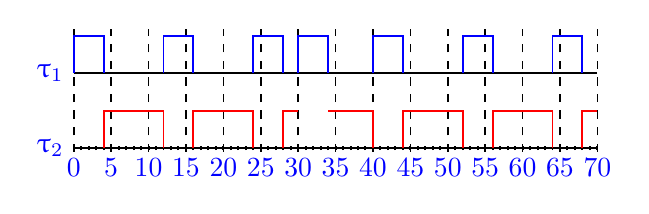
\begin{tikzpicture}[
		scale=0.095,
		line width=0.25mm,
		every node/.style={scale=1, text=blue},
		major tick/.style={semithick, dashed},
		x tick label/.style={anchor=north, minimum width=5mm},
		task1/.style={blue},
		task2/.style={red},
		task3/.style={green},
		desc/.style={anchor=east}
		]
	
	% Task 2
	\draw (0, 0) -- (70, 0);
	\node[desc] at (0, 0) {$\uptau_2$};
	
	% Task 1
	\draw (0, 10) -- (70, 10);
	\node[desc] at (0, 10) {$\uptau_1$};	
	
	% Small ticks
	\foreach \x in {0, 1,...,70}{
		\draw (\x, -0.25) -- (\x, 0.25);
	}
	
	% Major ticks with label
	\foreach \x/\label in {0, 5,...,70}{
		\node[x tick label] at (\x, 0) {$\label$}; 		
		\draw[major tick] (\x, -0.5) -- (\x, 16);
	}
	
	% Draw all
%	\foreach \x in {0, 10,...,69}{
%		\draw[task1] (\x, 10) -- (\x, 15) -- (\x+4, 15) -- (\x+4, 10);
%	}

	\draw[task1] (0, 10) --  (0, 15) --  (4, 15) -- (4, 10);
	\draw[task2] (4, 0) --  (4, 5) --  (12, 5) -- (12, 0);
	\draw[task1] (12, 10) --  (12, 15) --  (16, 15) -- (16, 10);
	\draw[task2] (16, 0) --  (16, 5) --  (24, 5) -- (24, 0);
	\draw[task1] (24, 10) --  (24, 15) --  (28, 15) -- (28, 10);
	\draw[task2] (28, 0) --  (28, 5) --  (30, 5); % 2 done
	\draw[task1] (30, 10) --  (30, 15) --  (34, 15) -- (34, 10);
	\draw[task2] (34, 5) --  (40, 5) -- (40, 0);	
	\draw[task1] (40, 10) --  (40, 15) --  (44, 15) -- (44, 10);
	\draw[task2] (44, 0) --  (44, 5) --  (52, 5) -- (52, 0);
	\draw[task1] (52, 10) --  (52, 15) --  (56, 15) -- (56, 10);
	\draw[task2] (56, 0) --  (56, 5) --  (64, 5) -- (64, 0);
	\draw[task1] (64, 10) --  (64, 15) --  (68, 15) -- (68, 10);
	\draw[task2] (68, 0) --  (68, 5) --  (70, 5);
		
	\end{tikzpicture}
%	\caption{Ablaufübersicht}
\end{figure} 
\end{frame}

\begin{frame}{\subsecname}
	Aber:\pause
	\begin{itemize}
		\item Zieht man den Aufwand der Context-Switches in Betracht ergibt sich ein anderes Bild
	\end{itemize}
\end{frame}

\begin{frame}{\subsecname}
	Context-Switching/Preemptions:
	\begin{itemize}
		\item Umschalten zwischen verschiedenen Tasks
		\item Zieht Aufwände mit sich
	\end{itemize}
\end{frame}

\begin{frame}{\subsecname}
	Rate Monotonics:
	\begin{figure}[htbp]
	% Partly taken from http://www.texample.net/tikz/examples/convolution-of-two-functions/
	\centering
	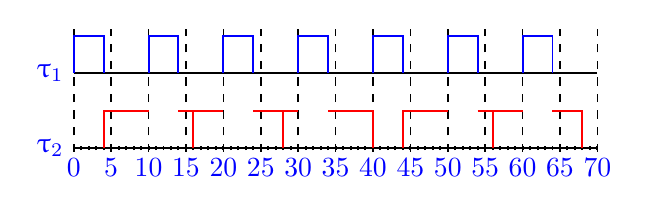
\begin{tikzpicture}[
		scale=0.095,
		line width=0.25mm,
		every node/.style={scale=1, text=blue},
		major tick/.style={semithick, dashed},
		x tick label/.style={anchor=north, minimum width=5mm},
		task1/.style={blue},
		task2/.style={red},
		task3/.style={green},
		desc/.style={anchor=east}
		]
	
	% Task 2
	\draw (0, 0) -- (70, 0);
	\node[desc] at (0, 0) {$\uptau_2$};
	
	% Task 1
	\draw (0, 10) -- (70, 10);
	\node[desc] at (0, 10) {$\uptau_1$};	
	
	% Small ticks
	\foreach \x in {0, 1,...,70}{
		\draw (\x, -0.25) -- (\x, 0.25);
	}
	
	% Major ticks with label
	\foreach \x/\label in {0, 5,...,70}{
		\node[x tick label] at (\x, 0) {$\label$}; 		
		\draw[major tick] (\x, -0.5) -- (\x, 16);
	}
	
	% Draw all
%	\foreach \x in {0, 10,...,69}{
%		\draw[task1] (\x, 10) -- (\x, 15) -- (\x+4, 15) -- (\x+4, 10);
%	}

	\draw[task1] (0, 10) --  (0, 15) --  (4, 15) -- (4, 10);	
	\draw[task2] (4, 0) -- (4, 5) -- (10, 5);
	\draw[task1] (10, 10) -- (10, 15) -- (14, 15) -- (14, 10);
	\draw[task2] (14, 5) -- (16, 5) -- (16, 0);
	\draw[task2] (16, 0) -- (16, 5) -- (20, 5);
	\draw[task1] (20, 10) -- (20, 15) -- (24, 15) -- (24, 10);
	\draw[task2] (24, 5) -- (28, 5) -- (28, 0);
	\draw[task2] (28, 0) -- (28, 5) -- (30, 5);
	\draw[task1] (30, 10) -- (30, 15) -- (34, 15) -- (34, 10);
	\draw[task2] (34, 5) -- (40, 5) -- (40, 0);
	\draw[task1] (40, 10) -- (40, 15) -- (44, 15) -- (44, 10);
	\draw[task2] (44, 0) -- (44, 5) -- (50, 5);
	\draw[task1] (50, 10) -- (50, 15) -- (54, 15) -- (54, 10);
	\draw[task2] (54, 5) -- (56, 5) -- (56, 0);
	\draw[task2] (56, 0) -- (56, 5) -- (60, 5);
	\draw[task1] (60, 10) -- (60, 15) -- (64, 15) -- (64, 10);
	\draw[task2] (64, 5) -- (68, 5) -- (68, 0);
		
	\end{tikzpicture}
%	\caption{Ablaufübersicht}
\end{figure} 
	Erliest Deadline First:
	\begin{figure}[htbp]
	% Partly taken from http://www.texample.net/tikz/examples/convolution-of-two-functions/
	\centering
	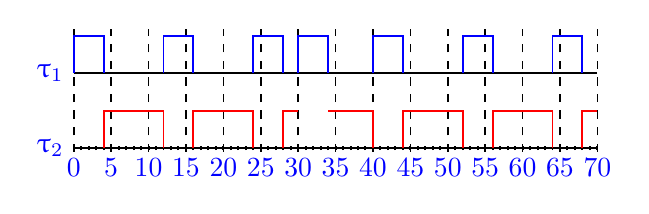
\begin{tikzpicture}[
		scale=0.095,
		line width=0.25mm,
		every node/.style={scale=1, text=blue},
		major tick/.style={semithick, dashed},
		x tick label/.style={anchor=north, minimum width=5mm},
		task1/.style={blue},
		task2/.style={red},
		task3/.style={green},
		desc/.style={anchor=east}
		]
	
	% Task 2
	\draw (0, 0) -- (70, 0);
	\node[desc] at (0, 0) {$\uptau_2$};
	
	% Task 1
	\draw (0, 10) -- (70, 10);
	\node[desc] at (0, 10) {$\uptau_1$};	
	
	% Small ticks
	\foreach \x in {0, 1,...,70}{
		\draw (\x, -0.25) -- (\x, 0.25);
	}
	
	% Major ticks with label
	\foreach \x/\label in {0, 5,...,70}{
		\node[x tick label] at (\x, 0) {$\label$}; 		
		\draw[major tick] (\x, -0.5) -- (\x, 16);
	}
	
	% Draw all
%	\foreach \x in {0, 10,...,69}{
%		\draw[task1] (\x, 10) -- (\x, 15) -- (\x+4, 15) -- (\x+4, 10);
%	}

	\draw[task1] (0, 10) --  (0, 15) --  (4, 15) -- (4, 10);
	\draw[task2] (4, 0) --  (4, 5) --  (12, 5) -- (12, 0);
	\draw[task1] (12, 10) --  (12, 15) --  (16, 15) -- (16, 10);
	\draw[task2] (16, 0) --  (16, 5) --  (24, 5) -- (24, 0);
	\draw[task1] (24, 10) --  (24, 15) --  (28, 15) -- (28, 10);
	\draw[task2] (28, 0) --  (28, 5) --  (30, 5); % 2 done
	\draw[task1] (30, 10) --  (30, 15) --  (34, 15) -- (34, 10);
	\draw[task2] (34, 5) --  (40, 5) -- (40, 0);	
	\draw[task1] (40, 10) --  (40, 15) --  (44, 15) -- (44, 10);
	\draw[task2] (44, 0) --  (44, 5) --  (52, 5) -- (52, 0);
	\draw[task1] (52, 10) --  (52, 15) --  (56, 15) -- (56, 10);
	\draw[task2] (56, 0) --  (56, 5) --  (64, 5) -- (64, 0);
	\draw[task1] (64, 10) --  (64, 15) --  (68, 15) -- (68, 10);
	\draw[task2] (68, 0) --  (68, 5) --  (70, 5);
		
	\end{tikzpicture}
%	\caption{Ablaufübersicht}
\end{figure} 
\end{frame}

\begin{frame}{\subsecname}
	Rate Monotonics:
	\begin{figure}[htbp]
	% Partly taken from http://www.texample.net/tikz/examples/convolution-of-two-functions/
	\centering
	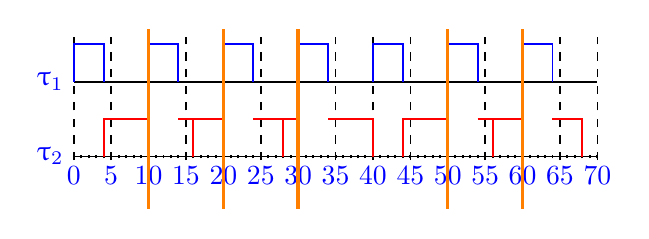
\begin{tikzpicture}[
		scale=0.095,
		line width=0.25mm,
		every node/.style={scale=1, text=blue},
		major tick/.style={semithick, dashed},
		x tick label/.style={anchor=north, minimum width=5mm},
		task1/.style={blue},
		task2/.style={red},
		task3/.style={green},
		desc/.style={anchor=east},
		konf/.style={orange, very thick}
		]
	
	% Task 2
	\draw (0, 0) -- (70, 0);
	\node[desc] at (0, 0) {$\uptau_2$};
	
	% Task 1
	\draw (0, 10) -- (70, 10);
	\node[desc] at (0, 10) {$\uptau_1$};	
	
	% Small ticks
	\foreach \x in {0, 1,...,70}{
		\draw (\x, -0.25) -- (\x, 0.25);
	}
	
	% Major ticks with label
	\foreach \x/\label in {0, 5,...,70}{
		\node[x tick label] at (\x, 0) {$\label$}; 		
		\draw[major tick] (\x, -0.5) -- (\x, 16);
	}
	
	% Draw all
%	\foreach \x in {0, 10,...,69}{
%		\draw[task1] (\x, 10) -- (\x, 15) -- (\x+4, 15) -- (\x+4, 10);
%	}

	\draw[task1] (0, 10) --  (0, 15) --  (4, 15) -- (4, 10);	
	\draw[task2] (4, 0) -- (4, 5) -- (10, 5);
	\draw[task1] (10, 10) -- (10, 15) -- (14, 15) -- (14, 10);
	\draw[task2] (14, 5) -- (16, 5) -- (16, 0);
	\draw[task2] (16, 0) -- (16, 5) -- (20, 5);
	\draw[task1] (20, 10) -- (20, 15) -- (24, 15) -- (24, 10);
	\draw[task2] (24, 5) -- (28, 5) -- (28, 0);
	\draw[task2] (28, 0) -- (28, 5) -- (30, 5);
	\draw[task1] (30, 10) -- (30, 15) -- (34, 15) -- (34, 10);
	\draw[task2] (34, 5) -- (40, 5) -- (40, 0);
	\draw[task1] (40, 10) -- (40, 15) -- (44, 15) -- (44, 10);
	\draw[task2] (44, 0) -- (44, 5) -- (50, 5);
	\draw[task1] (50, 10) -- (50, 15) -- (54, 15) -- (54, 10);
	\draw[task2] (54, 5) -- (56, 5) -- (56, 0);
	\draw[task2] (56, 0) -- (56, 5) -- (60, 5);
	\draw[task1] (60, 10) -- (60, 15) -- (64, 15) -- (64, 10);
	\draw[task2] (64, 5) -- (68, 5) -- (68, 0);
	
	\draw[konf] (10, 17) -- (10, -7);
	\draw[konf] (20, 17) -- (20, -7);
	\draw[konf] (30, 17) -- (30, -7);
	\draw[konf] (50, 17) -- (50, -7);
	\draw[konf] (60, 17) -- (60, -7);
		
	\end{tikzpicture}
%	\caption{Ablaufübersicht}
\end{figure} 
	Erliest Deadline First:
	\begin{figure}[htbp]
	% Partly taken from http://www.texample.net/tikz/examples/convolution-of-two-functions/
	\centering
	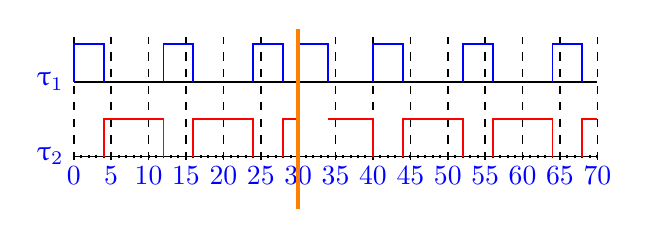
\begin{tikzpicture}[
		scale=0.095,
		line width=0.25mm,
		every node/.style={scale=1, text=blue},
		major tick/.style={semithick, dashed},
		x tick label/.style={anchor=north, minimum width=5mm},
		task1/.style={blue},
		task2/.style={red},
		task3/.style={green},
		desc/.style={anchor=east},
		konf/.style={orange, very thick}
		]
	
	% Task 2
	\draw (0, 0) -- (70, 0);
	\node[desc] at (0, 0) {$\uptau_2$};
	
	% Task 1
	\draw (0, 10) -- (70, 10);
	\node[desc] at (0, 10) {$\uptau_1$};	
	
	% Small ticks
	\foreach \x in {0, 1,...,70}{
		\draw (\x, -0.25) -- (\x, 0.25);
	}
	
	% Major ticks with label
	\foreach \x/\label in {0, 5,...,70}{
		\node[x tick label] at (\x, 0) {$\label$}; 		
		\draw[major tick] (\x, -0.5) -- (\x, 16);
	}
	
	% Draw all
%	\foreach \x in {0, 10,...,69}{
%		\draw[task1] (\x, 10) -- (\x, 15) -- (\x+4, 15) -- (\x+4, 10);
%	}

	\draw[task1] (0, 10) --  (0, 15) --  (4, 15) -- (4, 10);
	\draw[task2] (4, 0) --  (4, 5) --  (12, 5) -- (12, 0);
	\draw[task1] (12, 10) --  (12, 15) --  (16, 15) -- (16, 10);
	\draw[task2] (16, 0) --  (16, 5) --  (24, 5) -- (24, 0);
	\draw[task1] (24, 10) --  (24, 15) --  (28, 15) -- (28, 10);
	\draw[task2] (28, 0) --  (28, 5) --  (30, 5); % 2 done
	\draw[task1] (30, 10) --  (30, 15) --  (34, 15) -- (34, 10);
	\draw[task2] (34, 5) --  (40, 5) -- (40, 0);	
	\draw[task1] (40, 10) --  (40, 15) --  (44, 15) -- (44, 10);
	\draw[task2] (44, 0) --  (44, 5) --  (52, 5) -- (52, 0);
	\draw[task1] (52, 10) --  (52, 15) --  (56, 15) -- (56, 10);
	\draw[task2] (56, 0) --  (56, 5) --  (64, 5) -- (64, 0);
	\draw[task1] (64, 10) --  (64, 15) --  (68, 15) -- (68, 10);
	\draw[task2] (68, 0) --  (68, 5) --  (70, 5);
	
	\draw[konf] (30, 17) -- (30, -7);	
	
	\end{tikzpicture}
%	\caption{Ablaufübersicht}
\end{figure} 
\end{frame}

\begin{frame}{\subsecname}
	Fazit:
	\begin{itemize}
		\item Beachtet man den Aufwand der Context-Switches, erzeugt Rate Monotonics mehr Overhead als Erliest Deadline First
	\end{itemize}
\end{frame}


\subsection{Schedulability Analysis}
\begin{frame}{\subsecname}
	%TODO
\end{frame}

\subsection{Robustness During Overloads}\label{RobustnessDuringOverloads}

\begin{frame}{\subsecname}
	Mythos:
	\begin{itemize}
		\item Rate Monotonics ist in Overload-Situationen besser vorhersehbar
	\end{itemize}$ $\\\pause
	Szenarien:
	\begin{itemize}
		\item Permanent Overload
		\item Transient Overload
	\end{itemize}
\end{frame}

\subsubsection{Permanent Overload}
\begin{frame}{Beispiel Rate Monotonics}
	\begin{center}
		\begin{tabular}{c||c|c}
			Task ($\uptau_i$) & Dauer ($C_i$) & Task-Periode ($T_i$)\\\hline\hline
			$\uptau_1$ & 4 & 8\\
			$\uptau_2$ & 6 & 12\\
			$\uptau_3$ & 5 & 20
		\end{tabular}
	\end{center}
	\begin{figure}[htbp]
	% Partly taken from http://www.texample.net/tikz/examples/convolution-of-two-functions/
	\centering
	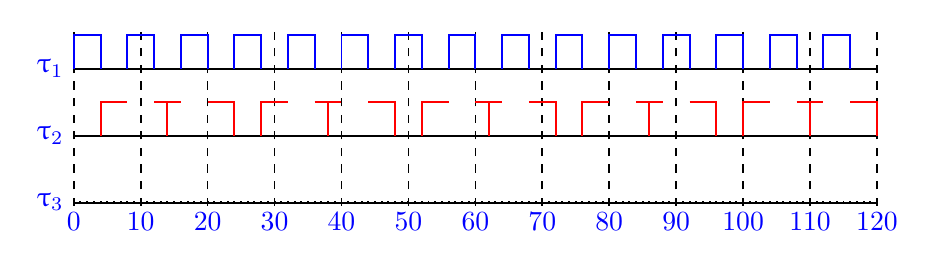
\begin{tikzpicture}[
		scale=0.085,
		line width=0.25mm,
		every node/.style={scale=1, text=blue},
		major tick/.style={semithick, dashed},
		x tick label/.style={anchor=north, minimum width=5mm},
		task1/.style={blue},
		task2/.style={red},
		task3/.style={green},
		desc/.style={anchor=east}
		]


	% Task 3
	\draw (0, 0) -- (120, 0);
	\node[desc] at (0, 0) {$\uptau_3$};
	
	% Task 2
	\draw (0, 10) -- (120, 10);
	\node[desc] at (0, 10) {$\uptau_2$};	

	% Task 1
	\draw (0, 20) -- (120, 20);
	\node[desc] at (0, 20) {$\uptau_1$};	

	
	% Small ticks
	\foreach \x in {0, 1,...,120}{
		\draw (\x, -0.25) -- (\x, 0.25);
	}
	
	% Major ticks with label
	\foreach \x/\label in {0, 10,...,120}{
		\node[x tick label] at (\x, 0) {$\label$}; 		
		\draw[major tick] (\x, -0.5) -- (\x, 26);
	}
	
	% Draw all
	\foreach \x in {0, 24,...,100}{
		\draw[task1] (\x, 20) -- (\x, 25) -- (\x+4, 25) -- (\x+4, 20);
		\draw[task2] (\x+4, 10) -- (\x+4, 15) -- (\x+8, 15);
		\draw[task1] (\x+8, 20) -- (\x+8, 25) -- (\x+12, 25) -- (\x+12, 20);
		\draw[task2] (\x+12, 15) -- (\x+14, 15) -- (\x+14, 10);
		\draw[task2] (\x+14, 10) -- (\x+14, 15) -- (\x+16, 15);
		\draw[task1] (\x+16, 20) -- (\x+16, 25) -- (\x+20, 25) -- (\x+20, 20);
		\draw[task2] (\x+20, 15) -- (\x+24, 15) -- (\x+24, 10);
	}

%	\draw[task1] (0, 10) --  (0, 15) --  (4, 15) -- (4, 10);	

		
	\end{tikzpicture}
%	\caption{Ablaufübersicht}
\end{figure} 
\end{frame}

\begin{frame}{Beispiel Erliest Deadline First}
	\begin{center}
		\begin{tabular}{c||c|c}
			Task ($\uptau_i$) & Dauer ($C_i$) & Task-Periode ($T_i$)\\\hline\hline
			$\uptau_1$ & 4 & 8\\
			$\uptau_2$ & 6 & 12\\
			$\uptau_3$ & 5 & 20
		\end{tabular}
	\end{center}
	\begin{figure}[htbp]
	% Partly taken from http://www.texample.net/tikz/examples/convolution-of-two-functions/
	\centering
	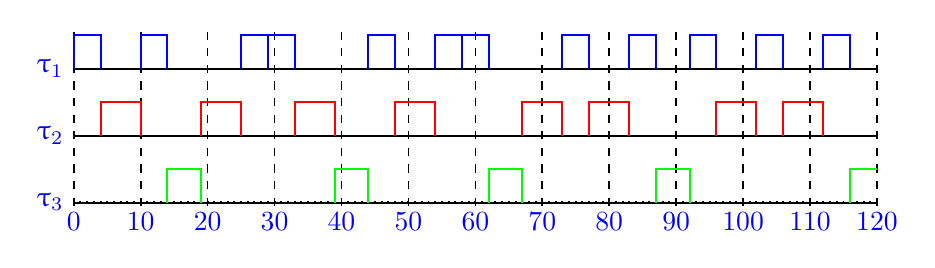
\begin{tikzpicture}[
		scale=0.085,
		line width=0.25mm,
		every node/.style={scale=1, text=blue},
		major tick/.style={semithick, dashed},
		x tick label/.style={anchor=north, minimum width=5mm},
		task1/.style={blue},
		task2/.style={red},
		task3/.style={green},
		desc/.style={anchor=east}
		]


	% Task 3
	\draw (0, 0) -- (120, 0);
	\node[desc] at (0, 0) {$\uptau_3$};
	
	% Task 2
	\draw (0, 10) -- (120, 10);
	\node[desc] at (0, 10) {$\uptau_2$};	

	% Task 1
	\draw (0, 20) -- (120, 20);
	\node[desc] at (0, 20) {$\uptau_1$};	

	
	% Small ticks
	\foreach \x in {0, 1,...,120}{
		\draw (\x, -0.25) -- (\x, 0.25);
	}
	
	% Major ticks with label
	\foreach \x/\label in {0, 10,...,120}{
		\node[x tick label] at (\x, 0) {$\label$}; 		
		\draw[major tick] (\x, -0.5) -- (\x, 26);
	}

	\draw[task1] (0, 20) --  (0, 25) --  (4, 25) -- (4, 20);
	\draw[task2] (4, 10) --  (4, 15) --  (10, 15) -- (10, 10);
	\draw[task1] (10, 20) --  (10, 25) --  (14, 25) -- (14, 20);
	\draw[task3] (14, 0) --  (14, 5) --  (19, 5) -- (19, 0);
	\draw[task2] (19, 10) --  (19, 15) --  (25, 15) -- (25, 10);
	\draw[task1] (25, 20) --  (25, 25) --  (29, 25) -- (29, 20);
	\draw[task1] (29, 20) --  (29, 25) --  (33, 25) -- (33, 20);
	\draw[task2] (33, 10) --  (33, 15) --  (39, 15) -- (39, 10);
	\draw[task3] (39, 0) --  (39, 5) --  (44, 5) -- (44, 0);
	\draw[task1] (44, 20) --  (44, 25) --  (48, 25) -- (48, 20);
	\draw[task2] (48, 10) --  (48, 15) --  (54, 15) -- (54, 10);
	\draw[task1] (54, 20) --  (54, 25) --  (58, 25) -- (58, 20);
	\draw[task1] (58, 20) --  (58, 25) --  (62, 25) -- (62, 20);
	\draw[task3] (62, 0) --  (62, 5) --  (67, 5) -- (67, 0);
	\draw[task2] (67, 10) --  (67, 15) --  (73, 15) -- (73, 10);
	\draw[task1] (73, 20) --  (73, 25) --  (77, 25) -- (77, 20);
	\draw[task2] (77, 10) --  (77, 15) --  (83, 15) -- (83, 10);
	\draw[task1] (83, 20) --  (83, 25) --  (87, 25) -- (87, 20);
	\draw[task3] (87, 0) --  (87, 5) --  (92, 5) -- (92, 0);
	\draw[task1] (92, 20) --  (92, 25) --  (96, 25) -- (96, 20);
	\draw[task2] (96, 10) --  (96, 15) --  (102, 15) -- (102, 10);
	\draw[task1] (102, 20) --  (102, 25) --  (106, 25) -- (106, 20);
	\draw[task2] (106, 10) --  (106, 15) --  (112, 15) -- (112, 10);
	\draw[task1] (112, 20) --  (112, 25) --  (116, 25) -- (116, 20);
	\draw[task3] (116, 0) --  (116, 5) --  (120, 5);
	
	\draw[task3] (14, 0) --  (14, 5) --  (19, 5) -- (19, 0);
		
	\end{tikzpicture}
%	\caption{Ablaufübersicht}
\end{figure} 
\end{frame}

\begin{frame}{Beispiel}
	\begin{figure}[htbp]
	% Partly taken from http://www.texample.net/tikz/examples/convolution-of-two-functions/
	\centering
	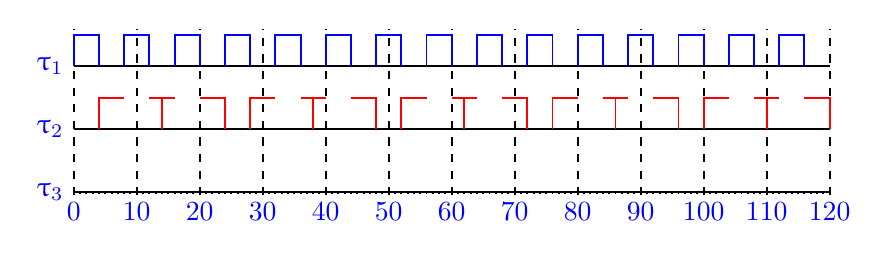
\begin{tikzpicture}[
		scale=0.08,
		line width=0.25mm,
		every node/.style={scale=1, text=blue},
		major tick/.style={semithick, dashed},
		x tick label/.style={anchor=north, minimum width=5mm},
		task1/.style={blue},
		task2/.style={red},
		task3/.style={green},
		desc/.style={anchor=east}
		]


	% Task 3
	\draw (0, 0) -- (120, 0);
	\node[desc] at (0, 0) {$\uptau_3$};
	
	% Task 2
	\draw (0, 10) -- (120, 10);
	\node[desc] at (0, 10) {$\uptau_2$};	

	% Task 1
	\draw (0, 20) -- (120, 20);
	\node[desc] at (0, 20) {$\uptau_1$};	

	
	% Small ticks
	\foreach \x in {0, 1,...,120}{
		\draw (\x, -0.25) -- (\x, 0.25);
	}
	
	% Major ticks with label
	\foreach \x/\label in {0, 10,...,120}{
		\node[x tick label] at (\x, 0) {$\label$}; 		
		\draw[major tick] (\x, -0.5) -- (\x, 26);
	}
	
	% Draw all
	\foreach \x in {0, 24,...,100}{
		\draw[task1] (\x, 20) -- (\x, 25) -- (\x+4, 25) -- (\x+4, 20);
		\draw[task2] (\x+4, 10) -- (\x+4, 15) -- (\x+8, 15);
		\draw[task1] (\x+8, 20) -- (\x+8, 25) -- (\x+12, 25) -- (\x+12, 20);
		\draw[task2] (\x+12, 15) -- (\x+14, 15) -- (\x+14, 10);
		\draw[task2] (\x+14, 10) -- (\x+14, 15) -- (\x+16, 15);
		\draw[task1] (\x+16, 20) -- (\x+16, 25) -- (\x+20, 25) -- (\x+20, 20);
		\draw[task2] (\x+20, 15) -- (\x+24, 15) -- (\x+24, 10);
	}

%	\draw[task1] (0, 10) --  (0, 15) --  (4, 15) -- (4, 10);	

		
	\end{tikzpicture}
%	\caption{Ablaufübersicht}
\end{figure} 
	\begin{figure}[htbp]
	% Partly taken from http://www.texample.net/tikz/examples/convolution-of-two-functions/
	\centering
	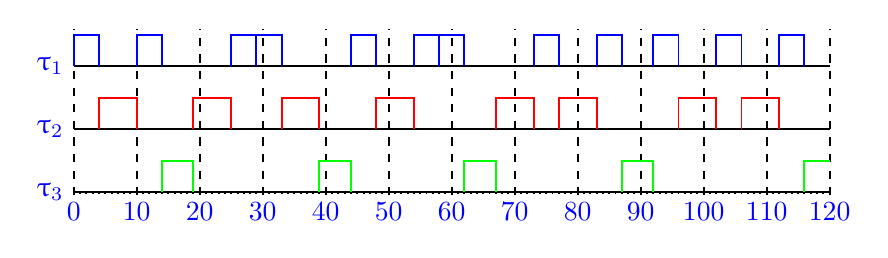
\begin{tikzpicture}[
		scale=0.08,
		line width=0.25mm,
		every node/.style={scale=1, text=blue},
		major tick/.style={semithick, dashed},
		x tick label/.style={anchor=north, minimum width=5mm},
		task1/.style={blue},
		task2/.style={red},
		task3/.style={green},
		desc/.style={anchor=east}
		]


	% Task 3
	\draw (0, 0) -- (120, 0);
	\node[desc] at (0, 0) {$\uptau_3$};
	
	% Task 2
	\draw (0, 10) -- (120, 10);
	\node[desc] at (0, 10) {$\uptau_2$};	

	% Task 1
	\draw (0, 20) -- (120, 20);
	\node[desc] at (0, 20) {$\uptau_1$};	

	
	% Small ticks
	\foreach \x in {0, 1,...,120}{
		\draw (\x, -0.25) -- (\x, 0.25);
	}
	
	% Major ticks with label
	\foreach \x/\label in {0, 10,...,120}{
		\node[x tick label] at (\x, 0) {$\label$}; 		
		\draw[major tick] (\x, -0.5) -- (\x, 26);
	}

	\draw[task1] (0, 20) --  (0, 25) --  (4, 25) -- (4, 20);
	\draw[task2] (4, 10) --  (4, 15) --  (10, 15) -- (10, 10);
	\draw[task1] (10, 20) --  (10, 25) --  (14, 25) -- (14, 20);
	\draw[task3] (14, 0) --  (14, 5) --  (19, 5) -- (19, 0);
	\draw[task2] (19, 10) --  (19, 15) --  (25, 15) -- (25, 10);
	\draw[task1] (25, 20) --  (25, 25) --  (29, 25) -- (29, 20);
	\draw[task1] (29, 20) --  (29, 25) --  (33, 25) -- (33, 20);
	\draw[task2] (33, 10) --  (33, 15) --  (39, 15) -- (39, 10);
	\draw[task3] (39, 0) --  (39, 5) --  (44, 5) -- (44, 0);
	\draw[task1] (44, 20) --  (44, 25) --  (48, 25) -- (48, 20);
	\draw[task2] (48, 10) --  (48, 15) --  (54, 15) -- (54, 10);
	\draw[task1] (54, 20) --  (54, 25) --  (58, 25) -- (58, 20);
	\draw[task1] (58, 20) --  (58, 25) --  (62, 25) -- (62, 20);
	\draw[task3] (62, 0) --  (62, 5) --  (67, 5) -- (67, 0);
	\draw[task2] (67, 10) --  (67, 15) --  (73, 15) -- (73, 10);
	\draw[task1] (73, 20) --  (73, 25) --  (77, 25) -- (77, 20);
	\draw[task2] (77, 10) --  (77, 15) --  (83, 15) -- (83, 10);
	\draw[task1] (83, 20) --  (83, 25) --  (87, 25) -- (87, 20);
	\draw[task3] (87, 0) --  (87, 5) --  (92, 5) -- (92, 0);
	\draw[task1] (92, 20) --  (92, 25) --  (96, 25) -- (96, 20);
	\draw[task2] (96, 10) --  (96, 15) --  (102, 15) -- (102, 10);
	\draw[task1] (102, 20) --  (102, 25) --  (106, 25) -- (106, 20);
	\draw[task2] (106, 10) --  (106, 15) --  (112, 15) -- (112, 10);
	\draw[task1] (112, 20) --  (112, 25) --  (116, 25) -- (116, 20);
	\draw[task3] (116, 0) --  (116, 5) --  (120, 5);
	
	\draw[task3] (14, 0) --  (14, 5) --  (19, 5) -- (19, 0);
		
	\end{tikzpicture}
%	\caption{Ablaufübersicht}
\end{figure} 
\end{frame}

\begin{frame}{\subsubsecname}
	\begin{columns}[]
  			\begin{column}{0.5\textwidth}
				Rate Monotonics:
				\begin{itemize}
					\item Tasks mit langer Periode werden vollständig blockiert!
					\item Gut vorhersagbar
				\end{itemize}

			\end{column}
  			\begin{column}{0.5\textwidth}
  				Erliest Deadline First:
				\begin{itemize}
					\item Sieht chaotischer aus
					\item Durchschnittliche Periode $\bar{T}_i$ für einen Task $\uptau_i$ ist gegeben durch
						\begin{equation}
							\bar{T}_i=T_i\cdot U
						\end{equation}
				\end{itemize}	
  			\end{column}
	\end{columns}
\end{frame}

%\begin{frame}{\subsubsecname}
%	Beispiel mit EDF? %TODO
%\end{frame}

\begin{frame}{\subsubsecname}
	Fazit:
	\begin{itemize}
		\item Beide Verfahren bei permanenter Überlastung sehr gut vorhersagbar
		\item Einsatzgebiet ist stark Situationsabhängig
	\end{itemize}
\end{frame}

\subsubsection{Transient Overload}
\begin{frame}{\subsubsecname}
	Annahme für RM:
	\begin{itemize}
		\item Es werden Tasks mit kurzen Perioden bevorzugt\pause
		\item[$\Rightarrow$] Falls ein Task seine Deadline überschreitet, wird der Task mit der längsten Periodenlänge verschoben/unterbrochen	
	\end{itemize}
\end{frame}

\newcommand{\showRMSlideRob}[1] {\begin{frame}{\subsubsecname}
	\begin{center}
		\begin{tabular}{c||c|c}
			Task ($\uptau_i$) & Dauer ($C_i$) & Task-Periode ($T_i$)\\\hline\hline
			$\uptau_1$ & 6 & 15\\
			$\uptau_2$ & 9 & 27\\
			$\uptau_3$ & 3 & 60\\
			$\uptau_4$ & 3 & 90
		\end{tabular}
	\end{center}
	\input{graphics/vergleich/transient#1_RM.tex}
\end{frame}}

\forloop{ct}{1}{\value{ct} < 8}%
{%
	\showRMSlideRob{\arabic{ct}}
}

\begin{frame}{\subsecname}
	Fazit:
	\begin{itemize}
		\item Permanent Overload: Gleichwertig
		\item Transient Overload:
		\begin{itemize}
			\item Rate Monotonics verführt zu falschen Annahmen
		\end{itemize}
	\end{itemize}
\end{frame}

\begin{frame}{\subsecname}
	\begin{center}
			
\includegraphics[scale=1]{graphics/memes/busted.jpg}
	\end{center}
\end{frame}

\subsection{Jitter and Latency}

\begin{frame}{\subsecname}
	Beispiel für Jitter
\end{frame}

\begin{frame}{\subsecname}
	Vorurteil:
	\begin{itemize}
		\item Durch die festen Prioritäten entsteht währen der Laufzeit bei Rate Monotonics weniger Jitter als bei Erliest Deadline First. 
	\end{itemize}
\end{frame}

\begin{frame}{\subsecname}
	Beispiel aus Paper
\end{frame}

\begin{frame}{\subsecname}
	Graphen aus Paper
\end{frame}

\begin{frame}{\subsecname}
	Fazit:
	\begin{itemize}
		\item RM hält Jitter für die hoch priorisierten Tasks sehr niedrig, vernachlässigt jedoch die anderen Tasks
		\item Insgesamt erzeugt EDF, gerade bei hoher Auslastung, wesentlich weniger Jitter
	\end{itemize}
\end{frame}

\subsection{Other Issues}
\subsubsection{Ressource Sharing}
\begin{frame}{\subsubsecname}
	Test
\end{frame}

\subsubsection{Aperiodic Task Handling}
\begin{frame}{\subsubsecname}
	Test
\end{frame}

\subsubsection{Ressource Reservation}
\begin{frame}{\subsubsecname}
	Test
\end{frame}
	
	\section{Fazit}
	\begin{frame}{\secname}
	Vorteile von Rate Monotonics:\pause
	\begin{itemize}
		\item leichtere Implementierung in kommerziellen Systemen
		\item RTA benötigt weniger Schritte als PDC
	\end{itemize}\pause
	Vorteile Earliest Deadline First:\pause
	\begin{itemize}
		\item Erlaubt vertrauenswürdiges Scheduling solange $U \leq 1$
		\item Weniger Runtime Overhead
	\end{itemize}\pause
	Unentschieden oder Situationsabhängig:\pause
	\begin{itemize}
		\item Overload Situations
		\item Jitter Control
	\end{itemize}
\end{frame}

\begin{frame}{\secname}
	\begin{center}
		
\includegraphics[scale=0.35]{graphics/memes/success.jpg}
	\end{center}
\end{frame}


	
\begin{frame}{Fragen?}
	\begin{center}
			
\includegraphics[scale=.4]{graphics/memes/ask.jpg}
	\end{center}
\end{frame}
	
\end{document}